%%
%% This is file `example.tex',
%% generated with the docstrip utility.
%%
%% The original source files were:
%%
%% coppe.dtx  (with options: `example')
%% 
%% This is a sample monograph which illustrates the use of `coppe' document
%% class and `coppe-unsrt' BibTeX style.
%% 
%% \CheckSum{1613}
%% \CharacterTable
%%  {Upper-case    \A\B\C\D\E\F\G\H\I\J\K\L\M\N\O\P\Q\R\S\T\U\V\W\X\Y\Z
%%   Lower-case    \a\b\c\d\e\f\g\h\i\j\k\l\m\n\o\p\q\r\s\t\u\v\w\x\y\z
%%   Digits        \0\1\2\3\4\5\6\7\8\9
%%   Exclamation   \!     Double quote  \"     Hash (number) \#
%%   Dollar        \$     Percent       \%     Ampersand     \&
%%   Acute accent  \'     Left paren    \(     Right paren   \)
%%   Asterisk      \*     Plus          \+     Comma         \,
%%   Minus         \-     Point         \.     Solidus       \/
%%   Colon         \:     Semicolon     \;     Less than     \<
%%   Equals        \=     Greater than  \>     Question mark \?
%%   Commercial at \@     Left bracket  \[     Backslash     \\
%%   Right bracket \]     Circumflex    \^     Underscore    \_
%%   Grave accent  \`     Left brace    \{     Vertical bar  \|
%%   Right brace   \}     Tilde         \~}
%%
\documentclass[dsc,numbers]{coppe}
\usepackage{amsmath,amssymb}
\usepackage{hyperref}

% circuitos e tikz
\usepackage{tikz, tkz-euclide} 
\usepackage[europeanresistors,americaninductors]{circuitikz}
\usetikzlibrary{chains}
\usepackage{siunitx}
\usepackage{tikz-qtree}

\usepackage{pgfplots}

\pgfplotsset{compat=1.18}
%

\makelosymbols
\makeloabbreviations
\usepackage[dvipsnames]{xcolor} % letras coloridas

\begin{document}
  \title{T\'itulo da Tese}
  \foreigntitle{Thesis Title}
  \author{Nome do Autor}{Sobrenome}
  \advisor{Prof.}{Nome do Primeiro Orientador}{Sobrenome}{D.Sc.}
  \advisor{Prof.}{Nome do Segundo Orientador}{Sobrenome}{Ph.D.}
  \advisor{Prof.}{Nome do Terceiro Orientador}{Sobrenome}{D.Sc.}

  \examiner{Prof.}{Nome do Primeiro Examinador Sobrenome}{D.Sc.}
  \examiner{Prof.}{Nome do Segundo Examinador Sobrenome}{Ph.D.}
  \examiner{Prof.}{Nome do Terceiro Examinador Sobrenome}{D.Sc.}
  \examiner{Prof.}{Nome do Quarto Examinador Sobrenome}{Ph.D.}
  \examiner{Prof.}{Nome do Quinto Examinador Sobrenome}{Ph.D.}
  \department{PEC}
  \date{05}{2022}

  \keyword{Primeira palavra-chave}
  \keyword{Segunda palavra-chave}
  \keyword{Terceira palavra-chave}

  \maketitle

  \frontmatter
  \dedication{A algu\'em cujo valor \'e digno desta dedicat\'oria.}

  \chapter*{Agradecimentos}

  Gostaria de agradecer a todos.

  \begin{abstract}

  Apresenta-se, nesta tese, ...

  \end{abstract}

  \begin{foreignabstract}

  In this work, we present ...

  \end{foreignabstract}

  \tableofcontents
  \listoffigures
  \listoftables
  \printlosymbols
  \printloabbreviations

  \mainmatter
%%%%%%%%%%%%%%%%%%%%%%%%%%%%%%%%%%%%%%%%%%%%%%%%%%%%%%%%%%  

\chapter{Introdução} 
% 4 ítens
% (1)
  % Introdução sobre os temas tratados para pessoas que não são da área:
  % 1- O que é a eletrônica de potência e o seu papel para as tecnologias emergentes. 
  % 2- Indústria 
  % 3- A necessidade de agregar confiabilidade para a eletrônica de potência. O que é confiabilidade e sua relação histórica com a eletrônica de potência.
  % O sistema tratado no trabalho: O drive para o motor de indução.
  % O problema é que as soluções envolvendo eletrônica de potência se tornam cada vez mais difundidas em diversos setores da sociedade ao ponto que essa tecnologia passa a ser pensada como proposta fundamental para o desenvolvimento de áreas críticas como transportes, geração e transmissão de energia. Consequentemente, a segurança desses sistemas passa a depender cada vez mais da operação confiável da eletrônica de potência.

Atualmente, as aplicações que envolvem dispositivos com eletrônica de potência (EP) se difundem cada vez mais em diversos setores da indústria ao ponto de se tornarem facilitadoras para tecnologias emergentes em áreas críticas como a aviação, veículos elétricos (VE), geração e transmissão de energia. Tendo em vista a importância dessa tecnologia, este trabalho tem como o objetivo dissertar sobre as formas encontradas na literatura para agregar confiabilidade ao sistema formado por um motor de indução acoplado ao conversor de potência, os chamados \textit{motor drives}, e com o enfoque no uso dos sinais disponíveis previamente no sistema para o seu monitoramento e determinações de estados de falta que podem não ser percebidos pela proteção padrão. 

A EP, em termos gerais, tem a tarefa de processar e controlar o fluxo da energia ao suprir as correntes e tensões que são ótimas para a determinada carga. A natureza dessa tarefa demanda a menor perda de energia possível tanto pelo custo da energia perdida quanto pela dificuldade de remover o calor gerado pela perda. Outros fatores também se destacam como o custo, peso e tamanho reduzido para estes dispositivos. Essas demandas vem sendo satisfeitas com base nos avanços dos dispositivos semicondutores que podem ser operados de forma intermitente, isto é, a reproduzir padrões de abertura e fechamento em frequências altas. Isso resulta em uma operação com perdas inferiores às perdas ôhmicas, resistivas, que se resultariam em topologias da eletrônica comum.  

Os conversores de potência, dispositivos com EP para gerenciar alguma troca energética, possibilitaram melhorias no acionamento e controle de motores elétricos em um grande leque de aplicações: como compressores, bombas, precisão de posição e movimento em linhas de produção automatizadas, geração eólica, entre outros. Algumas das aplicações se destacam pela necessidade de sistemas com um grau de confiabilidade superior, ou seja, em que um defeito que leve a uma manutenção não programada ou uma falta catastrófica, envolve custos adicionais altos, perigo ao operador e perda de competitividade no mercado a depender da frequência de interrupção dos processos. 
% ilustrar o que é um drive

 Podemos ilustrar tais aplicações na área de aviação com o conceito de uma aviação mais elétrica (\textit{More Electric Aircraft} ou MEA). Esta indústria tem a característica da necessidade crescente da geração, ilustrada na Fig \ref{fig:aircrafttrends}, devido ao aumento do número de passageiros e a quantidade de equipamentos abordo.  O MEA tem a intensão de buscar por soluções de eficiência energética que estimulam a redução do consumo de combustível fóssil e peso total, através da implementação de mais recursos elétricos para abastecer os serviços a bordo. Atualmente, atende-se as demandas internas somente (sem a propulsão) \cite{MadonnaGiagrandeGalea2018}. Para que isso seja viável, o controle dos fluxos de energia dentro do avião precisam de equipamentos de alta performance, permitindo diagnósticos internos para planejar a manutenção, uma vez que ela só pode ser feita no solo.
 
\begin{figure}
\centering
\includegraphics[width=0.6\textwidth]{figuras/aircrafttrends.png}
\caption{\label{fig:aircrafttrends} Gráfico com a capacidade de geração de alguns dos modelos de aviões com o ano do projeto \cite{MoirSeabridgeJukes2013}.}
\end{figure}

Um outro exemplo são os Veículos elétricos (VE) e veículos elétricos híbridos (VEH) que tem conquistado espaço no mercado. Apesar da grande aplicação dos motores elétricos no século XX, a mobilidade elétrica foi superada pelos motores a combustão devido à capacidade energética superior dos combustíveis e, com isso, prover a locomoção por longas distâncias a preços menores. Entre os melhoramentos que favorecem a competitividade dos VE se destacam a forma de armazenamento de energia, os motores elétricos e a conciliação de uma EP de baixo custo, alta confiabilidade e densidade de potência \cite{Sarlioglu2017}. Em cenários futuros, como os prospectados por \cite{LiuChauWuGau2013}, a presença dos VEs é abordada como participantes da rede elétrica em um contexto de \textit{smart grids}, com muitas  possibilidade de trocas energéticas entre veículos e a rede através de conversores bidirecionais. A figura \ref{fig:v2g} exemplifica o cenário complexo das trocas energéticas promovidas por conversores de potência: figura \ref{fig:v2g}(a) representa as trocas entre carros e residências e a rede; figura \ref{fig:v2g}(b) representa pontos de recarga ligados a uma barra de média tensão.            

\begin{figure}
\centering
\includegraphics[width=0.6\textwidth]{figuras/v2g.png}
\caption{\label{fig:v2g} Cenário com várias possibilidades de trocas entre veículos elétricos e a rede \cite{LiuChauWuGau2013}.}
\end{figure}

Com isso, os exemplos relatados tem em comum que estão dentro da atual conjuntura de tecnologias emergentes, que buscam novas formas de gerar e usar a energia e que podem ser empregadas em situações exigentes. Por isso, há a necessidade de garantir a confiabilidade dos conversores de potência para que esses dispositivos possam ser empregados com o menos riscos ao sistema, pois as possíveis falhas ou execução precária recorrente reduzem a eficiência desejada e a vida útil dos equipamentos dependentes.

%(2)
\section{A Engenharia de Confiabilidade e a Eletrônica de Potência.}
A confiabilidade é a probabilidade de um item desenvolver a função exigida no tempo devido e em condições determinadas. Ela é frequentemente expressa pelo número de falhas em um período de tempo. A durabilidade é um aspecto da confiabilidade sobre capacidade de resistir aos mecanismos dependentes do tempo, como a fadiga e a corrosão, e pode ser expressa em tempo mínimo antes da ocorrência de um desgaste, segundo \cite{Patrick2011_2}.

Historicamente, o entendimento da engenharia de confiabilidade como uma disciplina foi possibilitado pelo desenvolvimento da estatística e o surgimento da produção em massa, isto é, a fabricação de bens de consumo em grandes quantidades  \cite{SALEH2006249}, com o propósito de prevenir a criação de falhas o quanto antes possível, como na fase de \textit{design}. Pois uma deficiência no \textit{design} tem efeito em todo os itens produzidos e o custo para a correção dos defeitos após a fabricação aumenta com a continuidade da produção. Desde a primeira metade do século XX, várias maneiras de abordar esse tópicos foram contempladas. Uma das vertentes que predominou até os anos 80, sobretudo nos Estados Unidos, foi a previsão de confiabilidade quantitativa, ou seja, baseada em dados de falhas coletadas e publicadas em manuais promovidos pelo departamento de defesa norte-americano e pela indústria. A sua principal premissa era que a confiabilidade do sistema dependia dos componentes que compõem o sistema e precisava de dados para compor modelos estatísticos de previsão, que asseguravam taxas de falhas constantes \cite{Denson98}. Isso era aceitável nos anos 60, nos primórdios da eletrônica, quando as taxas de falhas eram altas e os circuitos menos complexos.  

Com o avanço da tecnologia e a difusão de circuitos eletrônicos mais complexos, como os circuitos integrados, e de mais qualidade, ocorreu uma mudança de entendimento de causas das falhas dos sistemas em direção aos fatores ligados a sua aplicação, a fabricação, o \textit{design}, as exigências do sistema, interface e software, que não foram computados nesses modelos estatísticos antigos. Foi neste contexto que uma outra abordagem para a confiabilidade com base nos processos físicos pelos quais as falhas ocorrem, chamada de \cite{Physics-of-failure} ou POF, passou a ter mais evidência. Há artigos de revisão como o de \cite{HuaiWang2021} que discorrem sobre essa mudança de paradigma em direção a POF, ou seja, da relevância da análise e a modelagem dos mecanismos de falha de um sistema contando com as cargas submetidas durante o seu uso e os aspectos ambientais em que esse sistema está submetido. Através desses modelos, pode-se descobrir os elos frágeis no produto para que as recomendações no design, produção, controle de processo, teste e operação em campo possa ser proposta.   

%(3)
\subsection{A Eletrônica de potência em um período de mudança de paradigmas de confiabilidade.}
Atualmente, a abordagem de POF tem sido aplicada a microeletrônica por um pouco mais de 2 décadas e vários mecanismos de falha, ciclo de vida e foram estudados e manuais para orientar a análise da robustez em dispositivos eletrônicos foram publicados, como o exemplo do \cite{HandbookRobustness} voltado para a indústria automobilística. Segundo \cite{HuaiWang2021}, um dos fatores que fomentou esse desenvolvimento foi a busca por dispositivos eletrônicos \textit{off-the-shelf}, que são peças produzidas de maneira genérica para produtos eletrônicos maiores ou que são customizadas a partir da sua venda para o cliente na pós-produção. 

No entanto, apesar de relatos das pesquisas de POF voltadas para eletrônica de potência <fontes> e de confiabilidade de conversores, as experiências de aplicações como <fontes> revelaram que ao contrário da microeletrônica, a eletrônica de potência ainda vem praticando muito dos métodos convencionais dos manuais, com uma abordagem quantitativa estatística para a confiabilidade.     

A necessidade de uma mudança de paradigmas vem sendo reconhecida em diversas áreas, como na automobilística \cite{HandbookRobustness}, e as pesquisas continuam em desenvolvimento no presente, <fonte>. As experiências relatadas na área de microeletrônica podem contribuir como fundamentos para a área de eletrônica de potência. Contudo, muitos dos seus modelos físicos não são escaláveis para a eletrônica de potência, devido às diferentes cargas térmicas, interações entre componentes e suas conexões, como salienta \cite{HuaiWang2021}.

%(4)

% Topologia básica, sinais de corrente e tensão.
% Conversores de alto-desempenho são microprocessados.

%%%%%%%%%%%%%%%%%%%%%%%%%%%%%%%%%%%%%%%%%%%%%%%%%%%%%%%%%%

% 11 itens.
%(1)
% A insatisfação com relação ao monitoramento das condições em pesquisas.
% Demonstrar pesquisas de diferentes áreas sobre confiabilidade 
Nos últimos 30 anos foram coletados dados sobre o desempenho em diversos setores, como o de energia foto voltaica e eólica e análises foram com esse material, coletado em relatórios de campo ou através de questionários para as empresas. Esta sessão busca esclarecer as fragilidades encontradas em algumas dessas análises para compreender os desafios da eletrônica de potência. 

O trabalho de \cite{Boettcher2011} analisa um banco de dados, o <citar o nome> (WMEP), que contém informações sobre a operação e alguns relatórios de manutenção de turbinas eólicas na Alemanha no período de 1997 até 2005. Com 6400 relatórios de manutenção e cerca de 1500 turbinas eólicas que foram monitoradas por, ao menos, 10 anos cada é um dos bancos de dados mais importantes do setor. Um dos cuidados necessários ao analisar as informações sobre o setor eólico é identificar se há uma distinção entre os conceitos de turbinas eólicas empregadas, pois alguns deles, como o conceito dinamarquês usado nos primórdios, conecta a turbina diretamente na rede e não passa por eletrônica de potência. O WMEP possui essa distinção.

A figura \ref{figuras:WMEP} apresenta um gráfico com as principais causas de falhas relatadas para as potências entre 1 e 1,5 MW e acima de 1,5 MW.  Os dados analisados pelos autores não especificam um componente específico de falha mas apontam que o sistema elétrico envolveram cerca de 20\% do tempo de manutenção enquanto turbinas maiores que 1,5 MW superam os 30\% . Ao analisar, os autores argumentam que a confiabilidade das turbinas eólicas tendem a decrescer com o aumento da potência pois possuem mais componentes elétricos e, por isso, com mais chance de falha. Outro ponto é que o conceito dinamarquês de turbina prevalece entre as turbinas de 1 e 1,5 MW, ao passo que as turbinas com drives de velocidade variável prevalecem em potências maiores. O estudo também revela que as causas de manutenção foram de 35\% relacionadas à falhas de componentes, maior que os cerca 23\% relacionadas ao sistema de controle e os 19\% devido às intempéries.

\begin{figure}
\centering
\includegraphics[width=0.6\textwidth]{figuras/relacao de causas de falhas em turbinas eolicas WMEP.png}
\caption{\label{figuras:WMEP} A relação entre as causas de de manutenção em turbinas eólicas por WMEP \cite{Boettcher2011}}
\end{figure}

Outra pesquisa para saber sobre os requerimentos e as expectativas em relação aos conversores de potência em  setores como o automotivo, aeroespacial, energia elétrica, motor drives e fabricantes de componentes foi feita por \cite{ShaoyongY2011} em 2008. As respostas foram enviadas tanto por equipes que trabalham em escritórios quanto os responsáveis pela operação em fábricas e, entre os resultados, temos as medidas de confiabilidade adotadas, os componentes mais vulneráveis e a satisfação em relação ao  monitoramento dos dispositivos e a sua confiabilidade. Algumas das respostas são comentadas a seguir.

A correlação entre as medidas de confiabilidade adotadas de acordo com os agentes dos setores entrevistados estão reproduzidas na figura \ref{figuras:correlacaomedidasporsetor}. A utilização de supressores de tensão foram destacadas pelos fabricantes de componentes, enquanto o setor aeroespacial e de energia elétrica enfatizaram o uso de \textit{back up} e os setores automotivos e conversores para motores, a refrigeração. Os autores analisam que o setor de energia precisa de um alto ciclo de trabalho, 365 dias por ano, e a adoção de \textit{back up} de partes faz com que sua disponibilidade do serviço não seja prejudicada por uma falha; o setor de motores preferem aumentar a refrigeração do que dissipadores de calor maiores devido às exigências de potência; enquanto que os fabricantes de componentes, com diferentes prioridades, recomendam maiores dissipadores de calor e supressores de tensão.

\begin{figure}
\centering
\includegraphics[scale=0.6]{figuras/correlacaoconfiabilidadesetores.png}
\caption{\label{figuras:correlacaomedidasporsetor} A correlação entre as medidas de confiabilidade por setor \cite{ShaoyongY2011}}
\end{figure}

A correlação entre o custo da falha sobre o custo do sistema normal por setor é reproduzida na figura \ref{figuras:correlacaofalhaporsetor}. Podemos ver um custo baixo pela razão de falha no setor de energia, provavelmente pela capacidade do uso de redundâncias no sistema e a manutenção, como dito anteriormente. Enquanto o setores de conversores de motores e aeroespacial relatam uma alta razão de custo pela necessidade de interromper a produção e a dificuldade de manutenção, respectivamente.  

\begin{figure}
\centering
\includegraphics[width=0.6\textwidth]{figuras/correlacao entre falha por custo e o setor.png}
\caption{\label{figuras:correlacaofalhaporsetor} A correlação entre o custo da falha sobre o custo do sistema normal por setor \cite{ShaoyongY2011}}
\end{figure}

Outros padrões relevantes coletados são que o IGBT (Insulated Gate Bipolar Transistor) é a chaves semicondutoras mais empregadas; Os IGBTs, os capacitores e circuitos de disparo das chaves, os \textit{gate drivers} são os componentes mais frágeis citados; Os transientes do sistema são as prováveis principais causas de falha destes dispositivos, seguidas pela sobrecarga e pelos efeitos ambientais, entre os quais se destacam a variação da temperatura.

Com isso, os resultados dessa pesquisa indicam que os métodos adotados para a confiabilidade do sistema dependem do setor de aplicação. Essencialmente, o investimento em confiabilidade se deve a aplicações críticas, que estão sujeitos a uma alta razão entre custo da falha pelo custo do sistema e que não tem um acesso fácil a manutenção ou capacidade de redundâncias. 


Por fim, o artigo de revisão \cite{Petrone2008} pesquisa sobre as questões relacionadas as plantas fotovoltaicas (FV) e aponta evidências de campo, como da Florida Solar Energy Center em \cite{Dhere2005}, que inclui informações sobre a operação de 103 sistemas FV conectados à rede, contendo um total de 176 inversores de quatro fabricantes e placas FV de 9 fabricantes, confirmam que a maior parte dos problemas relacionados a confiabilidade são devidos aos inversores. Em particular, os dados foram coletados de 1999 até 2003 registraram 213 eventos dos quais 139 estão relacionados a interrupção não-intencional devido à faltas ou a manutenções não-programadas.

A sessão buscou entender melhor o problema da confiabilidade entre vários agentes do mercado através dos relatos de pesquisas. As informações apresentadas ressaltam que há uma questão com a confiabilidade dos conversores devido a serem relacionados como a parte mais frágil do sistema ou de preocupação por parte das indústrias. As porcentagens mostradas não deve ser tomadas como definitivas, pois há diferença no tempo e na forma de coleta dos dados entre cada pesquisa. Apenas que uma das tendências é para a busca de melhoramentos na forma de monitoramento das condições do sistema, o assunto em que se fundamenta este trabalho.

\section{Descrição do sistema estudado}
A estrutura básica de um sistema de conversão eletromecânica de energia pode ser representada na figura tal em que há uma fonte, uma etapa de conversão de energia e um motor. Esta estrutura é comumente chamada de \textit{motor drive} na literatura e seu o objetivo é que o motor proporcione o padrão de movimento necessário para a atividade. Esta seção contém os assuntos para o entendimento de cada elemento do sistema a fim de fundamentar as tecnologias referidas nestes capítulo de revisão bibliográfica e no Métodos.

\subsection{Motor de Indução}
O funcionamento de um motor elétrico de corrente alternada se baseia na lei de Faraday, em que se um fluxo magnético passa por uma bobina, uma tensão será induzida nos terminais da bobina que é diretamente proporcional à taxa de variação do fluxo magnético com relação ao tempo. Caso a bobina esteja em um circuito fechado, a tensão será induzida de forma que produza uma corrente que gere um fluxo tal que se oponha ao campo magnético (lei de Lenz). 

A interação entre dois campos magnéticos em uma máquina elétrica, o do rotor e do estator da máquina, produz um torque para que esses campos se alinhem, se anulando. Então, a ideia por traz da construção de um motor elétrico é ter um campo gerado pela corrente no estator de tal forma que se combine com o campo do rotor e que produza um campo resultante que induza constantemente um torque no rotor. Para isso, o campo resultante do estator deve ter a direção variante no tempo, devido a forma do motor. Por essa razão que o textos da área chamam esse campo resultante de girante \cite{Chapman4}. Uma das formas de ter esse efeito é através de uma alimentação com 3 correntes alternadas defasadas de $120^o$, o dito sistema trifásico com a frequência $\omega$.  
\begin{align} 
    I_A(t) &= I_M sin(\omega t)  &[A] \label{eq:IfaseA}\\
    I_B(t) &= I_M sin(\omega t - 120º) &[A] \label{eq:IfaseB}\\ 
    I_C(t) &= I_M sin(\omega t + 120º) &[A] \label{eq:IfaseC}
\end{align}
Pode-se ver o campo girante resultante através da explicação de \cite{Chapman4}, reproduzido na figura tal. A figura representa um estator vazio em que as correntes da fase A, B e C estão presentes nas bobinas indicadas por aa', bb' e cc', equações \ref{eq:IfaseA}, \ref{eq:IfaseB} e \ref{eq:IfaseC},  respectivamente.

Devido a corrente alternada, a densidade de campo $B$ para cada fase terá uma direção fixa, mas com intensidade variável. O ângulo após cada equação é devido ao referencial adotado na figura.
\begin{align}
    B_{aa'} &= B_M sin(\omega t) \angle 0^o &[T] \label{eq:HfaseA}\\
    B_{bb'} &= B_M sin(\omega t - 120º) \angle 120^o &[T] \label{eq:HfaseB} \\
    B_{cc'} &= B_M sin(\omega t + 120º) \angle 240^o &[T] \label{eq:HfaseC} 
\end{align}
O campo resultante é calculado pela equação \ref{eq:campogirante} a seguir. 
\begin{equation}
    B_{res} = B_{aa'} + B_{bb'} + B_{cc'}    
\end{equation}
A resultante será: % trocar essa equação por um desenho.
\begin{equation}
    B_{res} = 1,5 B_M sin(\omega t) \hat{x} - 1,5B_M cos(\omega t) \hat{y} \label{eq:campogirante}
\end{equation}
O campo resultante para a configuração de bobinas obtido na figura tal possui módulo constante e direção variável no tempo, com velocidade angular $\omega$ obtida da rede. Em um motor real, o campo resultante é distribuído espacialmente no entreferro. Supondo que o rotor seja cilíndrico, a relutância do entreferro é muito maior que a do estator e do rotor e, por isso, o campo percorre o menor caminho entre os dois e os flui de forma perpendicular às superfícies. Essa configuração também requer uma distribuição senoidal dos condutores das bobinas pelos espaços para que a densidade de campo magnético no entreferro além das correntes trifásicas. Mesmo com essas considerações, a configuração prática apenas se aproxima de uma distribuição senoidal mesmo com o sistema equilibrado, pois há um número finito de condutores e espaços para o encaixe deles e distorções no sinal de corrente podem ser observadas.

% falar sobre o torque e os efeitos da má qualidade do sinal 
\subsubsection{Torque induzido no rotor}
Parte da potência transferida no entreferro ao rotor é perdida e parte se transforma em movimento do rotor através do torque induzido. Em textos como \cite{Chapman7}, O torque de um motor de indução é deduzido com a ajuda do circuito equivalente por fase, como podemos ver na figura \ref{fig:circuitoporfase}. O torque, equação \ref{eq:torqueinduzido}, depende da corrente de fase ($I_1$), dos componentes do circuito por fase, do escorregamento ($s$) e da frequência ($\omega$). 
\begin{equation}\label{eq:torqueinduzido}
    \tau_{ind} = f(I_1, \omega, s)
\end{equation}
\begin{figure}
    \centering
\begin{circuitikz}[american]
    %% Def dos pontos
    \tkzDefPoints{0/0/A,
                  0/3/B,
                  5/3/C,
                  5/0/D,
                  8/3/E,
                  8/0/F,
                  2/3/B1,
                  6/3/C1};
    %% circuito
    % tensão inicial
    \draw (A) to [open, l = $V_\phi$, voltage = straight, *-*] (B);
    % sinal +
    \draw (-0.5,2.25) -- ++(0.5,0);
    \draw (-0.25,2.0) -- ++(0,0.5);
    % sinal -
    \draw (-0.5,0.5) -- ++(0.5,0);
    
    \draw (B) to[R, l = $R_1$, i = $I_1$] (B1);
    \draw (B1) to[inductor, l = $jX_1$] (C);
    \draw (C) to[inductor, l = $jX_M$] (D);
    \draw (D) -- (A);
    \draw (C) to [inductor, l = $jX_2$, i = $I_2$] (E);
    \draw (E) to [R, l = $R2/s$] (F);
    \draw (F) -- (D);
\end{circuitikz}    
    \caption{Circuito equivalente por fase do motor de indução. }
    \label{fig:circuitoporfase}
\end{figure}

\subsection{Conversor}

\subsection{Controle}
A tecnologia mais comum dos conversores com velocidade variável é baseada nos inversores com modulação por largura de pulso (\textit{Pulse Width Modulation} ou (PWM)). Em primeiro, a corrente alternada da fonte é retificada, ou seja, transformada em corrente contínua em um elo CC, e, em seguida, a corrente alternada é fornecida ao motor através de 6 chaves semicondutoras como mostra a figura tal, essa etapa é chamada de inversão. A potência fornecida ao motor é regulada através do padrão de abrir e fechar cada uma das chaves. 
%(2)
\section{Os Principais Mecanismos de Degradação nos IGBTs.}
As chaves semicondutoras são dispositivos que combinam camadas de semicondutores com níveis de diferentes dopagem  para ativar um fluxo de elétrons entre seus terminais sob determinadas condições. Um exemplo do esquema básico do IGBT pode ser visto na figura \ref{fig:IGBT} de \cite{malvino2015}. As regiões indicadas por \textit{p} na figura se referem à presença de receptores de cargas negativas, "buracos" na camada de valência; e a indicação \textit{n}, à regiões com excesso de cargas negativas, os elétrons.

\begin{figure}
\centering
\includegraphics[scale = 0.7]{figuras/IGBTbasico.png}
\caption{\label{fig:IGBT} Esquema básico de um IGBT \cite{malvino2015}.}
\end{figure}

O IGBT é controlado por uma tensão \( V_{GE} \) positiva maior que o limiar de potencial do dispositivo \(V_{GE0}\), em que GE corresponde aos terminais \textit{Gate-Emitter}. Uma vez que a tensão é estabelecida, um efeito de campo atrai os elétrons livres da camada \(n^+\) superior até o terminal do Gate, mas eles não completam o caminho devido à camada isolante, geralmente de dióxido de silício (\(SiO_2\)). Consequentemente, a tensão promove a condução dos elétrons no sentido \textit{Emitter-Colector} quando esses terminais estão conectados a um circuito com malha fechada \cite{malvino2015}.        

Os blocos de camadas semicondutoras (chip) são inseridos em módulos de potência com diversas tecnologias. Enquanto o chip fornece o funcionamento básico do dispositivo, os módulos proveem as conexões elétricas, dissipação de calor, proteção contra o ambiente e manuseio. Segundo \cite{Hyunseok2015}, há dois tipos de módulos que são amplamente difundidos: O encapsulamento que contém um contato com fio de alumínio, que chamaremos de módulo com fio de alumínio (MFA) e o encapsulamento com contatos a pressão, que chamaremos de módulo com contatos a pressão (MCP). 

O MFA é a tecnologia de encapsulamento mais difundida e é ilustrado nas figuras \ref{fig:bondwiremodule} e \ref{fig:bondwiremodule2}. A primeira ilustração, de \cite{Hyunseok2015}, mostra o encapsulamento final com a presença dos terminais e o gel de silício (\textit{encapsulant}) para dissipação térmica e isolamento elétrico; a outra, de \cite{Rozanov2016}, mostra o módulo acoplado a uma unidade de refrigeração, usualmente a água, ar ou ventilação. Já o MCP, figura \ref{fig:presspack}, elimina um dos mecanismos de falhas presentes no MFA, originados no fio de alumínio, e possui vantangens como uma melhor dissipação de calor e maior resistência a curto-circuitos \cite{Hyunseok2015}.

\begin{figure}
\centering
\includegraphics[scale = 0.6]{figuras/bondwiremodule.png}
\caption{\label{fig:bondwiremodule} Módulo com contatos de alumínio entre os terminais \cite{Hyunseok2015}.}
\end{figure}

\begin{figure}
\centering
\includegraphics[scale = 0.6]{figuras/bondwiremodule2.png}
\caption{\label{fig:bondwiremodule2} Módulo com contatos de alumínio entre os terminais acoplado a uma unidade de refrigeração \cite{Rozanov2016}.}
\end{figure}

Os mecanismos de degradação dependem da tecnologia do módulo de potência em que o chip é instalado. Logo, uma dificuldade em definir assertivamente todos os mecanismos é que o avanço tecnológico trabalha para coibir os meios de falhas frequentes mas pode gerar novos e desconhecidos. Os possíveis mecanismos podem surgir devido a degradação do material com o uso ou sobrecargas elétricas, térmicas ou mecânicas. Neste trabalho, abordaremos alguns mecanismos mais frequentes encontrados na literatura com relação às fadigas na solda, a deterioração da condutividade térmica e sobrecargas elétricas para o IGBT do tipo MFA com o fim de modelar alguns deles em simulações da pesquisa.

\begin{figure}
\centering
\includegraphics[scale = 0.7]{figuras/presspack.png}
\caption{\label{fig:presspack} Módulo com contatos a pressão \cite{Hyunseok2015}.}
\end{figure}

\subbusection{Fadigas na solda}
O mecanismo de falha surge no contato entre materiais diferentes que são soldados dentro do módulo. A solda conecta dois materiais com coeficientes de expansão térmicas (CET) diferentes sujeitos aos ciclos térmicos do dispositivo durante a sua vida útil. Logo, surgem tensões que degradam a solda com o tempo. Em casos extremos, ocorre a ruptura da solda. Uma região de falha frequente em MFA é a degradação do contato do fio de alumínio com a interface do chip (de silício). O defeito é conhecido na literatura como \textit{bondwire lift off}  e é mostrado na figura \ref{fig:bondwirelift} em que o fio se desconecta da superfície de contato causando circuito-aberto \cite{Yang2010} ou um aumento na resistência do circuito.

\begin{figure}
\centering
\includegraphics[scale=0.6]{figuras/bondwireliftoff.png}
\caption{\label{fig:bondwirelift} Caso extremo do desgaste da solda no fio de alumínio causa o descolamento da placa \cite{Yang2010}.}
\end{figure}    

Semelhantes defeitos podem ocorrer em outras interfaces soldadas do módulo, como entre o substrato e a base ou o substrato e o chip. Elas começam com microestruturas que se desenvolvem em rachaduras e reduzem o contato entre as superfícies. O esquema da figura \ref{fig:solderfadigue} mostra os buracos que podem surgir devido a deterioração da solda no chip e que se tornam empecilhos para a dissipação térmica. 

\begin{figure}
\centering
\includegraphics[width=0.6\textwidth]{figuras/solderfadigue.png}
\caption{\label{fig:solderfadigue} Esquema de desgaste da solda na interface do chip com o substrato \cite{Yang2010}.}
\end{figure}

Segundo o artigo \cite{Wuchen1995}, uma outra possibilidade relatada é a eletromigração induzida pelo efeito da dissipação do calor no fio de alumínio.  Esse fenômeno se caracteriza pela deposição de alumínio na superfície do chip como se fosse um derretimento do fio provocado pelos estresses térmicos.  

\subsubsection{Deterioração da condutividade térmica.}
Entre a base do circuito e o aparelho dissipador há uma pasta com alta condutividade térmica. A sua função é distribuir o calor gerado no módulo e garantir a redução máxima da temperatura do chip. A deterioração da pasta ocorre com os ciclos térmicos do dispositivo e por sua interface entre dois materiais de CET diferentes. Isso resulta em um aumento da impedância térmica que irá reduzir a dissipação de calor \cite{Narumanchi2008}. A redução da dissipação de calor, por sua vez, influencia no aumento da temperatura da junção P-N (\(T_j\)) no chip.

O aumento da temperatura da junção P-N além do limite máximo do dispositivo reduz a capacidade de condução de corrente na área de operação segura (AOS) com a possibilidade de catalisar um curto-circuito mesmo em regime normal de operação \cite{BALIGA2015}. Devido a importância da dissipação de calor, uma tendência do setor automotivo são os módulos de potência com duplo dissipador de calor, como no trabalho de \cite{MA2021} mostrado na figura \ref{fig:doublesidedcooler}.

\begin{figure}
\centering
\includegraphics[width=0.6\textwidth]{figuras/doublesidedcooler.png}
\caption{\label{fig:doublesidedcooler} Módulo de potência com tecnologia press pack e duplo dissipador de calor de \cite{MA2021}.}
\end{figure}

\subsubsection{Sobrecarga Elétrica}
Os efeitos da exposição do dispositivo fora da AOS podem catalisar diversos mecanismos de falha no módulo e no chip com a sobrecorrente ou sobretensão e o aquecimento gerado na operação.

Na região do módulo de potência, o gel de silicone presente no encapsulamento, pode ter suas propriedades dielétricas reduzidas devido a uma sobretensão. Com isso, há a possibilidade de aparecer micro-espaços gasosos dentro da cápsula e a ocorrência de descargas elétricas parciais nesses pontos e erosão \cite{Fabian2005}, contribuindo para a destruição do módulo. Outro efeito é a ação de ampliar as fadigas existentes nas soldas devido à temperatura imposta pela sobrecarga.

No chip, a sobrecarga contribui para o aumento da \(T_j\) que pode catalisar um curto-circuito entre o \textit{collector} e \textit{emitter}. O termo \textit{burnout} geralmente é associado ao curto-circuito após um tempo de degradação do dispositivo. As partes que dissipam a energia da corrente de curto são, principalmente, o chip (semicondutor) e fio de alumínio, no MFA. Logo, a sobrecorrente no fio pode produzir um arco que percorre um caminho de corrente alternativo no módulo e a onda de choque se propaga pelo gel de silicone, que ocasiona a destruição do dispositivo \cite{Mauro2002}. 

% Colocar uma figura
Outro efeito relatado é que o colapso repentino da sobretensão \(V_{CE}\) (dV/dt) pode ativar o tiristor parasita dentro do dispositivo e, com isso, curto-circuitar o \textit{collector}, \textit{emitter} e o \textit{gate} \cite{Mauro2002}. No entanto, é um fenômeno relacionado com a robustez do dispositivo, ou seja, a capacidade de resistir à condições além da AOS.

%(3)

%(4)
\section{Análise das faltas de circuito aberto em um Conversor.}

\begin{figure}
\centering
\includegraphics[width=0.8\textwidth]{figuras/tipos de falhas.png}
\caption{\label{fig:tiposdefalhas} Os possíveis mecanismos de falhas na chave semicondutora IGBT \cite{Wu2013}}
\end{figure}

The failure mechanisms described in the previous sections can result in an open-circuit (OC) or short-circuit (SC) faults, they are summarized in the three diagram of the figure \ref{fig:tiposdefalhas} with the possible causes. The SC faults are difficult to deal with because the time between the fault initiation and the failure is small and needs precision and speed to avoid the catastrophic failures and, therefore, most of the detection mechanisms are based on hardware. This section is dedicated to analize the OC faults and their effects.

Show the event and the results as a DC offset.

How it effect the torque.

Open-circuit faults results in a DC offset in both the faulty and healthy phases. The interaction of the DC component and the field generates a pulsating torque at the stator current frequency which may reduce the average maximum torque available to the drive. 

Os primeiros indicadores para perceber o estado da chave foram os parâmetros elétricos da chave-semicondutora, como mostrado na tabela \ref{tab:indicadores}. Ao relacionar esses indicadores com os mecanismos de falha, os artigos de revisão como \cite{Hyunseok2015} e \cite{Yang2010} analisam que um mecanismo pode influenciar vários indicadores e que um só parâmetro pode não ser o suficiente para avaliar o estado do sistema. Por exemplo, o aumento de \(V_{CE,on}\) pode estar ligado à eletromigração de alumínio para a superfície do chip, devido da redução dos caminhos da corrente e consequente aumento da impedância, e pode estar relacionado a desconexão do mesmo fio; A deterioração da solda ou da camada de cerâmica, por sua vez, pode ocorrer com o aumento da impedância térmica \(R_{t}\). 

\begin{table}
\begin{center}
\begin{tabular}{|c | c|} 
 \hline
 Símbolo & Definição \\ [0.5ex] 
 \hline
 \(V_{CE,on}\) & Tensão coletor-emissor com a chave fechada (modo ligado). \\ 
 
  \(V_{GE}\) & Tensão gate-emissor. \\
 
 \(V_{GE,th}\) & Tensão limiar gate-emissor para o fechamento da chave. \\
 
 \(R_{t}\) & Impedância térmica do dispositivo. \\
 
 \(t_{off}\) & Tempo de abertura da chave. \\

 \(t_{on}\) & tempo de fechamento da chave \\ [1ex] 
 \hline
\end{tabular}
\caption{\label{tab:indicadores} Tabela com o resumo dos indicadores clássicos de acordo com \cite{Hyunseok2015}.}
\end{center}
\end{table}

O caminho para aferir os parâmetros elétricos da chave citados é através de hardware dedicado. Embora esse tipo de procedimento tenha relatos bem sucedidos de aplicações \textcolor{red}{fontes}, o presente trabalho busca entender as maneiras existentes de detecção de faltas e o monitoramento do estado através de sinais já disponíveis para o sistema de controle e proteção, como a corrente de saída do inversor.
% melhorar a sessão
%
Em um sistema trifásico equilibrado as tensões apresentam um comportamento senoidal com a diferença de fases de 120 graus e a aparência do sinal é similar ao da figura \textcolor{red}{tal}. No caso de um um inversor o sinal não é exatamente senoidal, mas com ruídos, como mostra o sinal de corrente na fase A da figura \ref{fig:Isanormal}.

\begin{figure}
\centering
\includegraphics[scale=0.6]{figuras/Isanormal.png}
\caption{\label{fig:Isanormal} Gráfico com a corrente do inversor na fase A.}
\end{figure}

As faltas CA em uma chave semicondutora podem ser causadas por algum problema em relação ao drive ou na própria chave como comentado na seção \textcolor{red}{tal}. Como vemos na chave F5 da figura \ref{fig:Inversor}, o problema no disparo da chave Q1 ocasiona em um estado inoperante da chave e ela não se fechará no tempo certo. Caso a falta seja de caráter intermitente, o sistema se recupera desse período transitório após um distúrbio no sinal da corrente  tal e representará um CA no sistema. O problema ressaltado por muitos autores, como \cite{Kastha1994}, é que o sistema de proteção convencional falha em averiguar a seriedade da falta. Por exmplo, caso o evento de CA aconteça durante uma carga leve, 

\begin{figure}
\centering
\includegraphics[scale=0.6]{figuras/inversorprovisorio.png}
\caption{\label{fig:Inversor} Esquema de um inversor com as chaves F5 e F6 para o CA e CC, respectivamente.}
\end{figure}

Uma das maneiras de entender as diferenças ocorridas no sinal de falta é através da transformação para o referencial estacionário \cite{Diallo2005}, chamado de \(\alpha-\beta\). A transformação 

O assunto de falta em um conversor vem sendo estudado há mais de 30 anos. Podemos ver artigos nos anos 90 sobre o assunto e propondo soluções. Alguns artigos na década de 90 propunham modelos matemáticos sobre faltas de caráter intermitente no conversor, tipo o tal. Com o avanço das pesquisas, a inteligência artificial 
%(6)
%(5)
\section{A Proteção de um Motor de Indução.}
%

\section{A revisão da literatura sobre o monitoramento das condições.}
%
\section{A review of the fault diagnostic methods.}
This section discuss the different approaches for OC fault diagnostics and their development through the last decade. The starting point is the review paper of \cite{BinSantosh09} which listed 21 strategies. The following topics group those methods and analyses their characteristics and the evolution of through the work of many authors.

\subsection{DC Offset Based Methods}
As explained in previous sections, the OC faults in a single transistor generates a DC offset between the fault and the healthy phase of the converter. Based on these features, the work of \cite{MendesCardoso09} introduced the fault detection and the defective switch location in a VSI with the average currents sampled at the inverter side.

First, the average over 1 period of the three-phase current signals \(\overline{I}_A\), \(\overline{I}_B\) and \(\overline{I}_C\) are calculated with their respectives phase angles.

\begin{equation}\label{eq:meancurrent}
    \overline{I}_{A,B,C} = |I_{A,B,C}|\angle \theta_{A,B,C}
\end{equation}

Given the sinusoidal nature of the current, a normal system has near 0 mean magnitude value. The degradation or anomalous conditions allow a DC offset in the signal which increases the average point's value. Hence, the Clarke's transform are applied to the currents as in equation \ref{eq:clarke}. 

\begin{equation}\label{eq:clarke}
    \begin{bmatrix}
    I_\alpha \\
    I_\beta
    \end{bmatrix} 
    = \sqrt{2/3} 
    \begin{bmatrix}
    1 & -1/2 & -1/2\\
    0 & \sqrt{3}/2 & \sqrt{3}/2
    \end{bmatrix}
    \begin{bmatrix}
    I_A\\
    I_B\\
    I_C
    \end{bmatrix}
\end{equation}

\begin{equation}\label{eq:alphabetadistance}
    |\overline{I}| = \sqrt{I_\alpha^2 + I_\beta^2}
\end{equation}

The Clarke's transformation maps the space fasor of the current signal onto a carthesian coordinate system known as the $\alpha\beta$-frame in the literature \cite{Yazdani10}. The events that damage the transistors increase the value of the $I_\alpha$ and $I_\beta$ gradually and its distance from the origin \ref{eq:alphabetadistance} increases. Experiments with a VSI drive with open loop control were made to determine the boundaries of the normal conditions for the current signals A, B, C, $|\overline{I}|$ and $\theta$ were made to determine where is the deffect and when it's triggered.

The load dependence is one of the algorithm's deficiency, because the higher the current fasor is, the higher its absolute value is affected by the degradation and moves further away the origin of the $\alpha\beta$ plane. Therefore, the thresholds need to be updated for each load. To solve this drawback, the work of \cite{RothenhagenFuchs05} normalizes the mean current value. This is achieved by computing the first order harmonic coefficients with the Discrete Fourier Transform (DFT) and dividing the mean value \ref{eq:meancurrent} by the absolute value of the first harmonic. The equation for the normalized current method is shown as follows:

\begin{equation}\label{eq:normalizedmeancurrent}
    \Tilde{I}_{A,B,C} = \frac{I_{A,B,C}}{\sqrt{a^2 + b^2}}\angle \theta_{A,B,C}
\end{equation}

The thresholds \ref{eq:Ithreshold1} and \ref{eq:Ithreshold2} were created by \cite{RothenhagenFuchs05} to improve the fault identification from the previous works and table \ref{tab:RothenhagenFuchs05Table} organizes the information of the thresholds and their respective transistor fault. 

\begin{equation}\label{eq:Ithreshold1}
d_1
\begin{cases}
    1: \Tilde{I}_i > 0\\
    0: \Tilde{I}_i <= 0
\end{cases}
\end{equation}

\begin{equation}\label{eq:Ithreshold2}
    d_2
    \begin{cases}
    1: |\Tilde{I}_i| > 0.45\\
    0: |\Tilde{I}_i| <= 0.45
    \end{cases}
\end{equation}

\begin{equation*}
    i \in \{A,B,C\}
\end{equation*}

\begin{table}
\centering
\begin{tabular}{|p{2cm}|p{1cm}|p{1cm}|p{1cm}|p{1cm}|p{1cm}|p{1cm}|}
\hline
Transistor & d_{1A} & d_{1B} & d_{1C} & d_{2A} & d_{2B} & d_{2C}\\[0.5ex]
\hline
  T1 & 1 & 0 & 0 & 1 & 0 & 0\\
\hline     
  T2 & 0 & 1 & 0 & 0 & 1 & 0\\
\hline
  T3 & 0 & 0 & 1 & 0 & 0 & 1\\
\hline
  T4 & 0 & 1 & 1 & 1 & 0 & 0\\
\hline
  T5 & 1 & 0 & 1 & 0 & 1 & 0\\
\hline
  T6 & 1 & 1 & 0 & 0 & 0 & 1\\
\hline 
\end{tabular}
    \caption{Table with values for the thresholds $d_1$ and $d_2$ and the respective transistor location. }
    \label{tab:RothenhagenFuchs05Table}
\end{table}

The authors also presented a modified version of this method to better perform under low currents, less than 10 $A_rms$, and with a close loop control. This modified normalized DC current method uses the same equations but with a less restrict classification of faults, reproduced in the table \ref{tab:RothenhagenFuchs05Table2}, where the blanks means that the value is neglected. Also, to prevent more than one condition fulfilled, only the largest absolute value among the currents at the time is used to analyse the thresholds.

\begin{table}
\centering
\begin{tabular}{|p{2cm}|p{1cm}|p{1cm}|p{1cm}|p{1cm}|p{1cm}|p{1cm}|}
\hline
Transistor & d_{1A} & d_{1B} & d_{1C} & d_{2A} & d_{2B} & d_{2C}\\[0.5ex]
\hline
  T1 & 1 &  &  & 1 &  & \\
\hline     
  T2 &  & 1 &  &  & 1 & \\
\hline
  T3 &  &  & 1 &  &  & 1\\
\hline
  T4 & 0 &  &  & 1 &  & \\
\hline
  T5 &  & 0 &  & & 1 & \\
\hline
  T6 &  &  & 0 &  &  & 1\\
\hline 
\end{tabular}
    \caption{Table with values for the thresholds $d_1$ and $d_2$ and the respective transistor location for the modified normalized DC current method.}
    \label{tab:RothenhagenFuchs05Table2}
\end{table}


%(8)
\subsection{Métodos baseados em dados e em \textit{Machine Learning}.}

%(9)
\subsection{O Monitoramento do conversor através das corrente de linha.}
A corrente do estator do motor pode ser usada para diferenciar o estado normal de operação do motor de um estado anormal. Primeiramente, as correntes de linha são medidas (\(I_{a}\), \(I_{b}\) e \(I_{c}\)) e, depois, precisamos extrair as informações necessárias para a classificação do estado. 
  
O trabalho de \cite{Diallo2005}, propôs a transformação das correntes de linha A,B e C para as coordenadas \(\alpha\) e \(\beta\). Em um padrão normal de atuação, as correntes nesse referencial compõem uma forma circular de eixos \(I_{\alpha}\) e \(I_{\beta}\).

%(10)
\section{Determinação da Vida útil restante e prognósticos.}
%

%(11)
\section{Resumos e comentários}
%

%%%%%%%%%%%%%%%%%%%%%%%%%%%%%%%%%%%%%%%%%%%%%%%%%%%%%%%%%%
\chapter{Revisão Bibliográfica}

\section{O Sistema em Estudo.}
A estrutura básica de um sistema de conversão eletromecânica de energia no âmbito deste trabalho pode ser representada na figura \ref{fig:sistema} em que há uma fonte, uma etapa de conversão de energia e um motor. Esta estrutura com um conversor-motor é comumente chamada de \textit{motor drive} na literatura e o seu objetivo é que o motor proporcione o padrão de movimento necessário para a atividade.

\begin{figure}
\centering
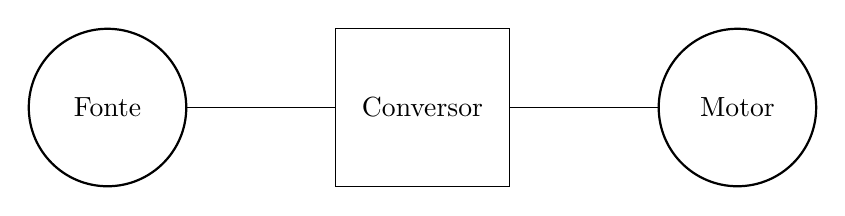
\begin{tikzpicture}
\node[circle,draw, minimum size = 2.0cm, thick](Fonte) at (0,0){Fonte};
\node[rectangle, draw, minimum width = 2.2cm, minimum height = 2.0cm](conv) at (4,0){Conversor};
\node[circle, draw, minimum size = 2.0cm, thick](motor) at (8,0){Motor};

\draw (Fonte) to[thick] (conv);
\draw (conv) to[thick] (motor);

\end{tikzpicture}
\caption{Sistema de conversão eletromecânica estudado.}
\label{fig:sistema}
\end{figure}

A fonte descrita na figura \ref{fig:sistema} pode representar o suprimento de energia em uma fábrica ou ambiente comercial em que o emprego do motor é necessário. Considera-se que ela fornece as tensões senoidais trifásicas e equilibradas, ou seja, tensões defasadas de 120º e com a mesma amplitude como nas equações a seguir.
\begin{align}
    V_a(t) &= V_M sin(\omega t) & [V] \\
    V_b(t) &= V_M sin(\omega t - 120^o) & [V] \\
    V_c(t) &= V_M sin(\omega t + 120^o) & [V] 
\end{align}

O motor do sistema funciona com a corrente alternada (CA) e pode ser aplicado em situações de velocidade variável, como, por exemplo, um veículo elétrico, em diversas máquinas na produção de papel,  máquinas da indústria têxtil, fabricação de cimento, linhas de produção de carros, etc. Tradicionalmente, as máquinas elétricas de CA foram usadas para aplicações com a frequência ou velocidade constante, enquanto as máquinas com corrente contínua (CC) foram preferidas para as aplicações com velocidades variáveis. Isso ocorreu devido à construção das máquinas CC que embora tenha desvantagens, como o maior custo por potência e problemas de manutenção com as escovas, possui um controle simples e a resposta do torque rápida. Por outro lado, as máquinas AC tem a construção mais robusta e um controle complexo. Essas questões motivaram muitas pesquisas sobre as aplicações de máquinas AC com a velocidade variável em conversores de potência \cite{Bose2}. Para o presente trabalho, o motor do sistema será o de indução. 
% Concertar essa figura.
\begin{figure}
    \centering
    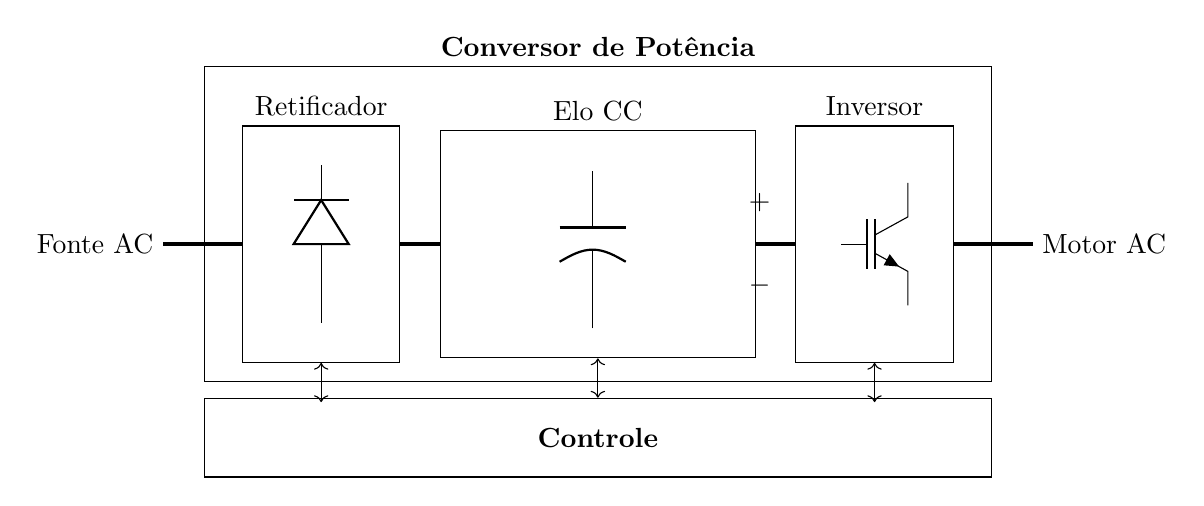
\begin{tikzpicture}[
	start chain = going right,
	box/.style = {
		on chain,join,draw,
		minimum height = 3cm,
		text centered,
		minimum width = 2cm,
	},
	every join/.style={ultra thick},
	node distance=5mm
]

\node [on chain] {Fonte AC}; % Chain starts here
\node [box, xshift=5mm, label = above: Retificador] (rec) {
	\begin{circuitikz}
		\draw (0,0) to[Do] (0,2);
	\end{circuitikz}
};

\node [on chain, join, draw, 
	text width=1cm,
	minimum width=4cm,
	minimum height=1.6cm,
	label=above:Elo CC,
] (ic) {
    \begin{circuitikz}[american voltages]
		\draw (0,0) to[pC, v<= $ $] (0,2);
	\end{circuitikz}
};

\node [box,label = above:Inversor] (inv) {
	\begin{circuitikz}
		\draw (0,0) node[nigbt] {};
	\end{circuitikz}
};

\node [on chain, join, xshift=5mm]{Motor AC};
% Chain ends here

% CU box
\node [
	rectangle,draw,
	below=5mm of ic,
	minimum width=10cm,
	minimum height=1cm,
] (cu) {\textbf{Controle}};

% PU box
\node [
	rectangle,draw,
	above=2mm of cu,
	minimum width=10cm,
	minimum height=4cm,
	label=\textbf{Conversor de Potência},
] (pu) {};

% Connections between CU and PU
\draw[<->] (rec.south) -- ++(0,-5mm);
\draw[<->] (cu.north) to (ic.south);
\draw[<->] (inv.south) -- ++(0,-5mm);

\end{tikzpicture}
    \caption{Diagrama de blocos com as diferentes partes de um conversor.}
    \label{fig:blocosdoconversor}
\end{figure}

O conversor conecta a fonte ao motor e, de uma forma geral, podemos descrever os seus componentes como a figura \ref{fig:blocosdoconversor}. A primeira etapa envolve a retificação do sinal através de uma "ponte" de diodo, figura \ref{fig:retificador}. Após a retificação, o elo CC, sustenta o nível de tensão através de um capacitor. Esse artifício torna o conversor alimentado por tensão, isto é, mantém-se a tensão para influenciar no sinal máximo a ser transmitido para o inversor. Por sua vez, o inversor funciona através da abertura e fechamento de chaves semi-condutoras na parte inversora e tem a corrente variável de acordo com as necessidades da carga. A topologia comum para o circuito trifásico pode ser vista na figura \ref{fig:inversor}.

\begin{figure}
    \centering
    \begin{circuitikz}
        % Pontos do circuitos
        \tkzDefPoints{ 0/2.5/A,
                       0/2.0/B,
                       0/1.5/C,
                       2/4/D,
                       2/2.5/E,
                       2/1.5/F,
                       2/0/G,
                       3.5/4/H,
                       3.5/2.5/I,
                       3.5/2.0/J,
                       3.5/1.5/K,
                       3.5/0/L,
                       5/4/M,
                       5/2.5/N,
                       5/1.5/O,
                       5/0/P,
                       6.5/4/Q,
                       6.5/0/R};
        % componentes
        \ctikzset{diodes/scale=0.6}
        \draw (E) to[D, l = D1] (D);
        \draw (G) to[D, l = D4] (F);
        \draw (L) to[D, l = D6] (K);
        \draw (I) to[D, l = D3] (H);
        \draw (P) to[D, l = D2] (O);
        \draw (N) to[D, l = D5] (M);
        \draw (R) to[C, v = $V_{CC}$] (Q);
        
        % conexões
        \draw (A) node[anchor = east]{A} to (E);
        \draw (E) -- (F);
        \draw (I) -- (J);
        \draw (J) -- (K);
        \draw (N) -- (O);
        \draw (B) node[anchor = east]{B} to (J);
        \draw (C) node[anchor = east]{C} to (O);
        \draw (D) -- (H);
        \draw (H) -- (M);
        \draw (M) -- (Q);
        \draw (G) -- (L);
        \draw (L) -- (P);
        \draw (P) -- (R);
        %\draw (
    \end{circuitikz}
    \caption{Topologia comum de uma ponte à diodo para retificação em um sistema trifásico.}
    \label{fig:retificador}
\end{figure}

\begin{figure}
    \centering
    \begin{circuitikz}[american]
    %% Definições dos pontos
    \tkzDefPoints{  0/0/A,
                    0/5/B,
                    2/5/C,
                    2/3/D,  %
                    2/0/E,
                    5/5/F,
                    5/2.5/G,%
                    5/0/H,
                    8/5/I,
                    8/2/J,  %
                    8/0/K,
                    2/4/t1,
                    2/1/t4,
                    5/4/t3,
                    5/1/t6,
                    8/4/t5,
                    8/1/t2,
                    11/2.5/M,
                    10/3/MA,
                    10/2.5/MB,
                    10/2/MC};
    %% componentes
    \draw (A) to[V, v=Vcc, invert] (B);
    \draw (t1) node[nigbt, bodydiode](T1){T1};
    \draw (t4) node[nigbt, bodydiode](T4){T4};
    \draw (t3) node[nigbt, bodydiode](T3){T3};
    \draw (t6) node[nigbt, bodydiode](T6){T6};
    \draw (t5) node[nigbt, bodydiode](T5){T5};
    \draw (t2) node[nigbt, bodydiode](T2){T2};
    \draw (M) node[elmech](M){M};
    
    %% ligações    
    \draw (B) -- (C);
    % leg A
    \draw (C) -- (T1.C);
    \draw (T1.E) -- (D);
    \draw (D) -- (T4.C);
    \draw (T4.E) -- (E);
    \draw (E) -- (A);
    % leg B
    \draw (F) -- (T3.C);
    \draw (T3.E) -- (G);
    \draw (G) -- (T6.C);
    \draw (T6.E) -- (H);
    \draw (H) -- (E);
    % leg C
    \draw (F) -- (I);
    \draw (I) -- (T5.C);
    \draw (T5.E) -- (J);
    \draw (J) -- (T2.C);
    \draw (T2.E) -- (K);
    \draw (C) -- (F);
    \draw (K) -- (H);
    % conectar ao motor
    \draw (D) -- (MA);
    \draw (MA) -- (M);
    \draw (G) -- (MB);
    \draw (MB) -- (M);
    \draw (J) -- (MC);
    \draw (MC) -- (M);
    
\end{circuitikz}
    \caption{Elo CC representado pela tensão $V_{CC}$ e a topologia comum de um inversor e suas conexões com o motor.}
    \label{fig:inversor}
\end{figure}

\subsection{O Papel da Proteção.}

A proteção para um \textit{drive} de velocidade variável, como descrito na sessão anterior, engloba os aspectos do próprio conversor e o motor associado. Para os \textit{drives} modernos, a maioria das funções de proteção são implementadas dentro do sistema de controle do conversor e com o foco na saída do sinal do conversor. Por isso, a proteção para a corrente na entrada (vinda da fonte) é comumente feita antes do conversor, próximo ao quadro de distribuição ou no centro de controle do motor, e inclui curto-circuito e faltas fase-terra. As principais funções de proteção que podem ser encontradas em um drive são \cite{BARNES2003}:

\begin{itemize}
    \item Subtensão CA na entrada do conversor;
    \item Subtensão CC no elo CC;
    \item Sobretensão CA na entrada do conversor;
    \item Sobretensão CC no elo CC;
    \item Sobrecorrente CA na saída do conversor;
    \item Falta fase-terra na saída do conversor;
    \item Altas temperatura no dissipador de calor;
    \item Sobrecarga térmica no motor.
\end{itemize}

As proteções contra subtensões tanto na entrada quanto no elo CC ocorrem apenas para certificar que o suprimento de energia está funcionando dentro das suas especificações, enquanto as proteções contra sobretensões e sobrecorrentes previnem os danos nos componentes do conversor. Assim como a sobrecorrente, as altas temperaturas, ocasionadas pelos ciclos de trabalho ou condições ambientais, limitam a vida útil dos semicondutores e a proteção garante que o sistema pare antes das faltas catastróficas, em que ocorre a destruição do equipamento.

A proteção contra faltas fase-terra é desenvolvida para detectar algum curto-circuito entre as fases e a terra. A sua função também é preservar o conversor e desconectar o equipamento assim que os limites são violados. Diferente das outras situações, a proteção fase-terra é usualmente implementada através de um transformador de corrente na saída do conversor. Esse dispositivo contém um núcleo toroidal magnético por onde as correntes passam e o secundário do transformador contém um circuito de baixa tensão que circula uma corrente caso a soma das correntes \( I_a\), \(I_b\) e \(I_c\) seja diferente de zero. 

A figura \ref{fig:protecaoConversor} ilustra as proteções citadas. Na entrada do conversor, os medidores calculam as tensões de linha \(V_{ab}\), \(V_{ac}\) e \(V_{bc}\) para a verificação de sobretensão e subtensão (SubT e SobT na figura); No elo CC, há medidores das tensões \(V_{CC}\) e correntes de linha \(I_{CC}\), para a verificação de sobretensão e sobrecorrente (CurtoC); Um sensor de temperatura verifica o estado das chaves semicondutoras (Temp).   
\begin{figure}
    \centering
    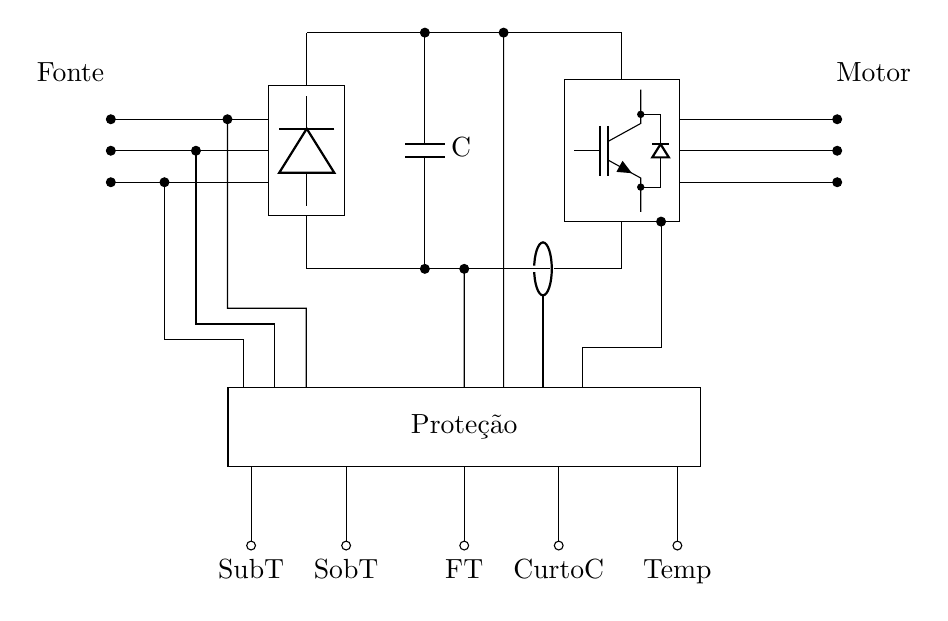
\begin{tikzpicture}
\tkzDefPoints{0/1/Ain,
              0/.5/Bin,
              0/0/Cin,
              2/1.5/A,
              3.5/1.5/B,
              4.5/1.5/C,
              6/1.5/D,
              2/-1.5/E,
              3.5/-1.5/F,
              5/-1.5/G,
              6/-1.5/H};

% retificador
\node [box,draw] at (2,0) (rec){
    \begin{circuitikz}
        \draw (0,0) to[D,scale = 0.7] (0,2);
    \end{circuitikz}
    };
    
% inversor    
\node [box, draw] at (6,0) (inv){
    \begin{circuitikz}
        \draw (0,0) node[nigbt, bodydiode]{};
    \end{circuitikz}
    };
    
\node [rectangle, draw,
       below = 15 mm of F,
       xshift = 5mm,
       minimum height = 1. cm,
       minimum width = 6 cm] (protec) {Proteção};

% conexões
\node[align = center] at (-1,1) {Fonte};
\node[align = center] at (9.2,1) {Motor};
\draw (rec.north) -- (A);
\draw (A) -- (B);
\draw (B) -- (D);
\draw (inv.north) --(D);
\draw (rec.south) -- (E);
\draw (E) -- (F);
\draw (F) -- ++(0.5,0);
\draw (F) ++(0.5,0) to[iloop, mirror, name = I] (H);
\draw (inv.south) -- (H);
\ctikzset{capacitors/scale=0.6};
\draw (B) to[C, l = C, *-*] (F);

\draw (rec.west) ++(0,0.4) to[short, -*] ++(-2,0);
\draw (rec.west) to [short, -*] ++(-2,0);
\draw (rec.west) ++(0,-0.4) to [short, -*] ++(-2,0);

\draw (inv.east) ++(0,0.4) to[short, -*] ++(2,0);
\draw (inv.east) to[short, -*] ++(2,0);
\draw (inv.east) ++(0,-0.4) to[short, -*] ++(2,0);

% conexões com o bloco da proteção.
\draw (protec.north) ++ (0.5,0) to [short, -*] (C);
\draw (F) ++ (0.5,0) to [short, *-] (protec.north) ++ (0.2,0);
\draw (protec.north) ++(1.5,0) to ++(0,0.5) to ++(1.,0) to [short,-*] ++(0,1.6);
\draw (protec.north) ++(1.,0) to (I.i);

\draw (protec.north west) ++(1.,0) to ++(0,1) to ++(-1.,0) to [short, -*] ++(0,2.4);
\draw (protec.north west) ++(.6,0) to ++(0,.8) to ++(-1.,0) to [short, -*] ++(0,2.2);
\draw (protec.north west) ++(.2,0) to ++(0,.6) to ++(-1.,0) to [short, -*] ++(0,2.);

% saída do bloco de proteção
\draw (protec.south west) ++(0.3,0) to ++(0,-1) node[ocirc, label = below:SubT]{};
\draw (protec.south) ++(-1.5,0) to ++(0,-1) node[ocirc, label = below: SobT]{};
\draw (protec.south) to ++(0,-1) node[ocirc, label = below: FT]{};
\draw (protec.south) ++(1.2,0) to ++(0,-1) node[ocirc, label = below: CurtoC]{};
\draw (protec.south east) ++(-0.3,0) to ++(0,-1) node[ocirc, label = below: Temp]{};
\end{tikzpicture}
    \caption{Esquema com as principais proteções para o conversor \cite{BARNES2003}.}
    \label{fig:protecaoConversor}
\end{figure}
% Incrementar com o livro do mamede e do coltrin.
% A diferença entre máquinas de grande porte e de pequeno porte.

\section{A Engenharia de Confiabilidade e a Eletrônica de Potência.}
% O que é
% Um pouco da história
% Subdivisões.
% Avanços.
A confiabilidade é a probabilidade de um item desenvolver a função exigida no tempo devido e em condições determinadas. Ela é frequentemente expressa pelo número de falhas em um período de tempo. Já a durabilidade é um aspecto da confiabilidade em relação a capacidade de resistir aos mecanismos dependentes do tempo, como a fadiga e a corrosão, e pode ser expressa em tempo mínimo antes da ocorrência de um desgaste, segundo \cite{Patrick2011_2}. A partir destas definições, esta seção se destina a entender um pouco do contexto histórico, as subdivisões e os avanços da área de engenharia de confiabilidade na eletrônica de potência.

\subsection{Contexto Histórico.}
O entendimento da engenharia de confiabilidade como uma disciplina foi possibilitado pelo desenvolvimento da estatística e o surgimento da produção em massa, isto é, a fabricação de bens de consumo em grandes quantidades \cite{SALEH2006249}, com o propósito de prevenir a criação de falhas o quanto antes possível, como na fase de \textit{design}. O motivo é que uma falha no \textit{design} tem efeito em todos os itens produzidos e o custo para a correção dos defeitos após a fabricação aumenta com a continuidade da produção. 

Uma das vertentes que predominou até os anos 80, sobretudo nos Estados Unidos, foram os métodos de previsão de confiabilidade quantitativa, ou seja, baseada em dados de falhas coletadas e publicadas em manuais providos pelo departamento de defesa norte-americano, como o MIL-HDBK-217F, e pela indústria. A principal premissa desses documentos era que a confiabilidade do sistema dependia dos componentes do sistema e precisava de dados de campo para os modelos estatísticos de previsão, que asseguravam taxas de falhas constantes \cite{Denson98}. 

As abordagens para a confiabilidade descritas no manual citado eram aceitáveis nos primórdios da eletrônica, quando as taxas de falhas eram altas e os circuitos menos complexos. Porém, com o avanço da tecnologia e a difusão de circuitos eletrônicos mais complexos, como os circuitos integrados, e de mais qualidade, cada vez mais evidências apontadas por especialistas da época sugeriam que o modelo de falha proposto pelo manual \cite{Denson98} não tinham precisão para prever as falhas e não eram atualizados para acompanhar o avanço tecnológico. Foi então que ocorreu uma mudança de entendimento gradual das causas das falhas dos sistemas em direção aos fatores ligados a sua aplicação, à fabricação, ao \textit{design}, às exigências do sistema, interface e software, que não foram computados nos modelos estatísticos antigos.

A partir desse cenário, uma outra abordagem para a confiabilidade com base nos processos físicos pelos quais as falhas ocorrem, chamada de \textit{Physics-of-failure} ou POF, passou a ter mais evidência. Há artigos de revisão como o de \cite{HuaiWang2021} que discorrem sobre essa mudança de paradigma em direção a POF, ou seja, da relevância da análise e a modelagem dos mecanismos de falha de um sistema contando com as cargas submetidas durante o seu uso e os aspectos ambientais em que esse sistema está submetido. Através desses modelos, pode-se descobrir os elos frágeis no produto para que as recomendações no design, produção, controle de processo, teste e operação em campo possam ser propostas.   

Por fim, através de uma linha temporal presente no trabalho de \cite{HuaiWang2021} e \cite{Chung2015}, figura \ref{fig:linhatemporal}, pode-se resumir os principais tópicos de pesquisas de cada época e fazer um paralelo entre a evolução da confiabilidade e da eletrônica de potência. A eletrônica de potência acompanhou o desenvolvimento das novas chaves semicondutoras, da possibilidade de produção e do controle e se beneficiou com os novos modelos para confiabilidade que surgiram no fim do século XX para suprir uma demanda da indústria e aplicações mais exigentes.

\begin{figure}
    \centering
    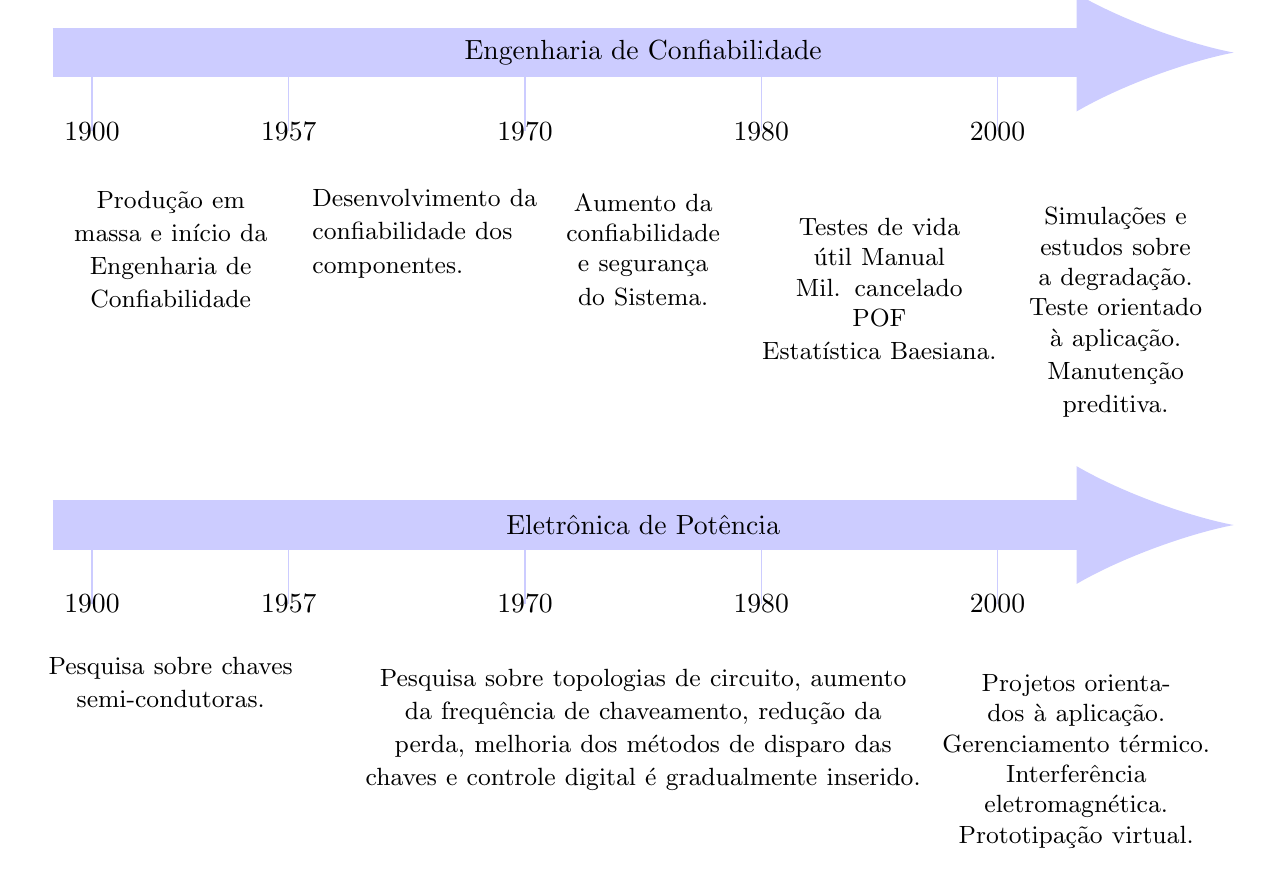
\begin{tikzpicture}
% textos da linha temporal da confiabilidade.
\node [align = center, text width = 3cm](texto1900) at (1.5, -2.5){\small Produção em massa e início da Engenharia de  Confiabilidade};
\node [align = left, text width = 3cm](texto1957) at (4.8, -2.3){ \small Desenvolvimento da confiabilidade dos componentes.};
\node [align = center, text width = 3cm](texto1970) at (7.5, -2.5){\small Aumento da confiabilidade e segurança \\\small do Sistema.};
\node [align = center, text width = 3.2cm](texto1980) at (10.5, -3.){\small Testes de vida útil Manual Mil. cancelado \\ \small POF\\ \small Estatística Baesiana.};
\node [align = center, text width = 3cm](texto2000) at (13.5, -3.3){\small Simulações e \\ \small estudos sobre a degradação. Teste orientado à aplicação.\\ \small Manutenção preditiva.};
%\draw[-{Triangle[width=18pt,length=8pt]}, line width=12pt](0,0) -- (15, 0);
\draw[->, >=latex, blue!20!white, line width=18pt] (0,0) to node[black]{Engenharia de Confiabilidade} (15,0);
\draw [blue!20!white](0.5,0.1) -- (0.5,-1.) node [black]{1900};
\draw [blue!20!white](3,0.1) -- (3,-1.) node [black]{1957};
\draw [blue!20!white](6,0.1) -- (6, -1.) node [black]{1970};
\draw [blue!20!white](9,0.1) -- (9, -1.) node [black]{1980};
\draw [blue!20!white](12,0.1) -- (12, -1) node [black]{2000};

% Textos da linha temporal de eletrônica de potência.
\node [align = center, text width = 3.2cm] at (1.5,-8){\small Pesquisa sobre chaves semi-condutoras.};
\node [align = center, text width = 7.2cm] at (7.5,-8.6){\small Pesquisa sobre topologias de circuito, aumento da frequência de chaveamento, redução da perda, melhoria dos métodos de disparo das chaves e controle digital é gradualmente inserido.};
\node [align = center, text width = 3.6cm] at (13,-9.0){\small Projetos orientados à aplicação. \\ \small Gerenciamento térmico. \\ \small Interferência eletromagnética. \\ \small Prototipação virtual. \\ };
\draw[->, >=latex, blue!20!white, line width=18pt] (0,-6) to node[black]{Eletrônica de Potência} (15,-6);
\draw [blue!20!white](0.5,-6.1) -- (0.5,-7.) node [black]{1900};
\draw [blue!20!white](3,-6.1) -- (3,-7.) node [black]{1957};
\draw [blue!20!white](6,-6.1) -- (6, -7.) node [black]{1970};
\draw [blue!20!white](9,-6.1) -- (9, -7.) node [black]{1980};
\draw [blue!20!white](12,-6.1) -- (12, -7) node [black]{2000};

\end{tikzpicture}

    \caption{Linha temporal de \cite{HuaiWang2021} e \cite{Chung2015} (adaptada) com os destaques da pesquisa da Eletrônica de Potência e da Engenharia de Confiabilidade por período de tempo no contexto desse trabalho.}
    \label{fig:linhatemporal}
\end{figure}

\subsection{A Pesquisa sobre a Confiabilidade em Eletrônica de Potência.}
Da perspectiva de \cite{Chung2015_2}, o futuro da pesquisa sobre confiabilidade em Eletrônica de Potência possui três pilares: A física analítica, design e verificação e controle e monitoramento. Esta seção descreve brevemente os conceitos desta perspectiva e ressalta o monitoramento das condições do conversor, a ênfase deste trabalho. 
\begin{figure}
    \centering
    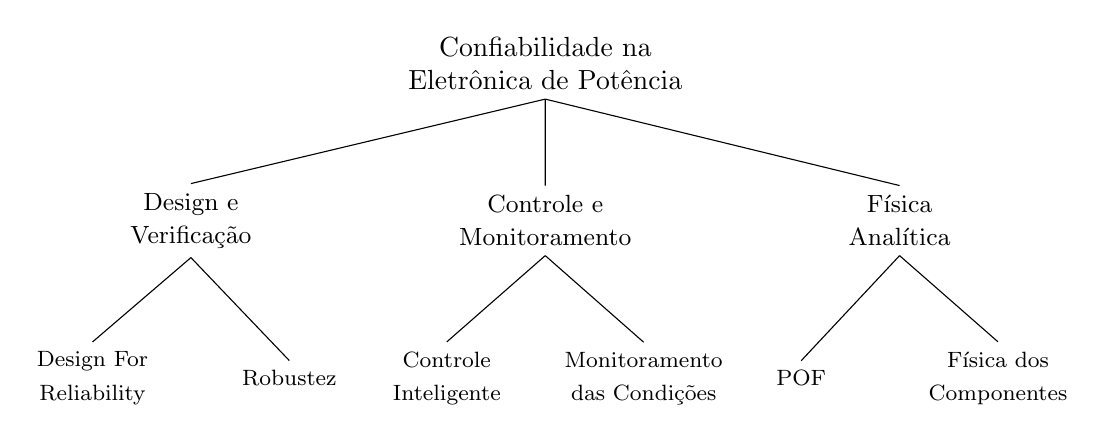
\begin{tikzpicture}
[
    level 1/.style = { sibling distance = 4.5cm},
    level 2/.style = { sibling distance = 2.5cm}
]
 
\node[align = center] {\normalsize Confiabilidade na\\\normalsize Eletrônica de Potência}[sibling distance = 2.cm, level distance = 2cm] 
    child [align = center]{node {\small Design e \\\small Verificação} child {node {\footnotesize Design For\\ \footnotesize Reliability}} 
    child {node {\footnotesize Robustez}}}
    child [align = center]{node {\small Controle e\\\small Monitoramento} child {node {\footnotesize Controle \\\footnotesize Inteligente}}
    child {node {\footnotesize Monitoramento \\\footnotesize das Condições}}}
    child [align = center]{node {\small Física\\\small Analítica}
    child {node {\footnotesize POF}}
    child {node {\footnotesize Física dos\\\footnotesize Componentes}}};
\end{tikzpicture}
    \caption{Os três pilares da pesquisa sobre Confiabilidade em Eletrônica de Potência.}
    \label{fig:pesquisaConfiabilidadeElePot}
\end{figure}

\subsubsection{Física Analítica}
O primeiro conceito necessário para uma eletrônica de potência mais confiável é entender a razão das falhas no nível do componente e dos sistemas através da sua análise física. A falha pode ocorrer de maneira súbita ou pela degradação no tempo. Pode-se entender a degradação do dispositivo no tempo através do esboço do gráfico da distribuição da capacidade do design (F) e das cargas (C) em que é submetido no ciclo de trabalho, como mostra a figura \ref{fig:degradacaonotempo}. O eixo x representa a carga (Por exemplo, temperatura, torque ou tensão) e o y, a frequência de aplicação de cada carga. Cada grandeza analisada pode ser alocada entre certos limites e representada por uma distribuição normal. Inicialmente, as cargas submetidas ao dispositivo estão respeitando os limites propostos pelo design a medida que nenhuma carga aplicada pode ser maior do que a capacidade do design. No entanto, a degradação atua de modo a enfraquecer o design por uma ação externa ou do próprio ciclo de trabalho até que uma parcela significativa da capacidade do design é afetada. Nesse ponto, determina-se o fim da vida útil do dispositivo. Isso implica que a falha pode ser adiada através de um aumento da capacidade do design ou pela aplicação da carga de forma reduzida com o tempo ou estado de degradação.   
\pgfmathdeclarefunction{gauss}{2}{%
  \pgfmathparse{1/(#2*sqrt(2*pi))*exp(-((x-#1)^2)/(2*#2^2))}%
}
\begin{figure}
    \centering
    
    \begin{tikzpicture}
\begin{axis}[
  no markers, domain=0:20, samples=100,
  axis lines*=left, xlabel=$x$, ylabel=$y$,
  every axis y label/.style={at=(current axis.above origin),anchor=south},
  every axis x label/.style={at=(current axis.right of origin),anchor=west},
  height=3.5cm, width=7.8cm,
  xtick={6,13.5}, ytick=\empty,
  enlargelimits=false, clip=false, axis on top,
  grid = major
  ]
  \addplot [very thick,cyan!50!black] {gauss(6,1)};
  \addplot [very thick,cyan!50!black] {gauss(13.5,1)};

\draw [yshift=-0.8cm, latex-latex](axis cs:10.5,0) -- node [fill=white] {F} (axis cs:16.5,0);
\draw [yshift=-0.8cm, latex-latex](axis cs:3.,0) -- node [fill=white] {C} (axis cs:9,0);

\end{axis}
\begin{axis}[yshift = 2.5cm, xshift = 1.79cm,
  no markers, domain=0:20, samples=100,
  axis lines*=left, xlabel=$x$, ylabel=$y$,
  every axis y label/.style={at=(current axis.above origin),anchor=south},
  every axis x label/.style={at=(current axis.right of origin),anchor=west},
  height=3.5cm, width=7.8cm,
  xtick={6,10.5}, ytick=\empty,
  enlargelimits=false, clip=false, axis on top,
  grid = major
  ]
    \addplot [fill=cyan!20, draw=none, domain=7.5:9] {gauss(6.,1)} \closedcycle;
  \addplot [very thick,cyan!50!black] {gauss(6,1)};
  \addplot [very thick,cyan!50!black] {gauss(10.5,1)};
  \end{axis}
  
  \begin{axis}[yshift = 5.cm, xshift = 3.5cm,
  no markers, domain=0:20, samples=100,
  axis lines*=left, xlabel=$x$, ylabel=$y$,
  every axis y label/.style={at=(current axis.above origin),anchor=south},
  every axis x label/.style={at=(current axis.right of origin),anchor=west},
  height=3.5cm, width=7.8cm,
  xtick={6,9.7}, ytick=\empty,
  enlargelimits=false, clip=false, axis on top,
  grid = major
  ]
  \addplot [fill=cyan!20, draw=none, domain=6.6:9] {gauss(6.,1)} \closedcycle;
  \addplot [very thick,cyan!50!black] {gauss(6,1)};
  \addplot [very thick,cyan!50!black] {gauss(9.7,1)};
  \addplot [very thick,magenta!30!white, dash pattern = on 3pt off 3pt] {gauss(13.5,1)};
  \end{axis}
  \draw [->](0,0) -- (55:7.cm);
  \draw (0,0) -- (55:3.5cm)node [ midway, above, sloped, align = center] (TextNode) {\small tempo};
  \draw [magenta!30!white,dash pattern=on 3pt off 3pt](3.3,0) -- +(55:6cm);
  \draw [magenta!30!white,dash pattern=on 3pt off 3pt](5.,0) -- +(55:6cm);
  \node [align = center](texto) at (8.6,3.5){Falta};
  \draw [->, thick, cyan!80!white, bend left = 20](texto.west) to +(155:2.3cm);
  \node [align = center](textoprojecao) at (8.8,7){Projeção};
  
\end{tikzpicture}
    \caption{Figura com a explicação para a falha através do tempo de serviço de \cite{Chung2015_2}. A legenda 'C' representa a carga do disposito e 'F' representa a força ´máxima suportável por design.}
    \label{fig:degradacaonotempo}
\end{figure}
% POF
\subsubsection{Design e Verificação}

\subsubsection{Controle e Monitoramento}
% Controle Inteligente
\subsection{O Monitoramento das Condições de um Conversor.}

\section{A Detecção de Faltas.}
\subsection{As faltas do ponto de vista dos IGBTs.}
\subsection{As faltas do ponto de vista do conversor.}
\subsection{As faltas do ponto de vista da fonte.}
\subsection{As faltas do ponto de vista do elo CC.}
\subsection{As faltas do ponto de vista do motor de indução.}

\section{Revisão Sobre a Detecção de Faltas de CA.}
\subsection{Os Caminhos de Detecção Através do Hardware.}
\subsection{Os Caminhos de Detecção Através do Software.}
\section{Resumo do Capítulo.}

%%%%%%%%%%%%%%%%%%%%%%%%%%%%%%%%%%%%%%%%%%%%%%%%%%%%%%%%%%
\chapter{Métodos}
\section{A Simulação}
Esse trabalho desenvolve um estudo sobre a detecção de faltas em um conversor controlador de um motor de indução trifásico. O estudo será por meio de simulação no ambiente do Simulink, através da biblioteca de \textit{Specialized Technology} dentro do d
\subsection{A configuração da proteção}
\subsection{O motor}
\subsection{O controle}
\subsection{Elo CC}


\section{O método para detecção de faltas}

\section{A determinação do estado normal e estado anormal de atuação.}

\section{Os casos estudados}

\chapter{Resultados e Discussões}
\section{Análise dos sinais de corrente nos casos estudados.}

\subsection{Possíveis efeitos no motor de Indução.}

\section{Detecção de faltas nas chaves semicondutoras.}

\subsection{Faltas do tipo circuito aberto.}

\subsection{Faltas de caráter intermitente no disparo drive.}

\section{Resumo do método proposto e seus resultados.}

%%%%%%%%%%%%%%%%%%%%%%%%%%%%%%%%%%%%%%%%%%%%%%%%%%%%%%%%%%
\chapter{Conclusões}

\backmatter
\bibliographystyle{coppe-unsrt}
\bibliography{Bibliografia}

\appendix
\chapter{Algumas Demonstra{\c c}\~oes}
\end{document}

